%%% Hlavní soubor. Zde se definují základní parametry a odkazuje se na ostatní části. %%%

%% Verze pro jednostranný tisk:
% Okraje: levý 40mm, pravý 25mm, horní a dolní 25mm
% (ale pozor, LaTeX si sám přidává 1in)
\documentclass[12pt,a4paper]{report}
\setlength\textwidth{145mm}
\setlength\textheight{247mm}
\setlength\oddsidemargin{15mm}
\setlength\evensidemargin{15mm}
\setlength\topmargin{0mm}
\setlength\headsep{0mm}
\setlength\headheight{0mm}
% \openright zařídí, aby následující text začínal na pravé straně knihy
\let\openright=\clearpage

%% Pokud tiskneme oboustranně:
% \documentclass[12pt,a4paper,twoside,openright]{report}
% \setlength\textwidth{145mm}
% \setlength\textheight{247mm}
% \setlength\oddsidemargin{14.2mm}
% \setlength\evensidemargin{0mm}
% \setlength\topmargin{0mm}
% \setlength\headsep{0mm}
% \setlength\headheight{0mm}
% \let\openright=\cleardoublepage

%% Vytváříme PDF/A-2u
\usepackage[a-2u]{pdfx}

%% Přepneme na českou sazbu a fonty Latin Modern
\usepackage[czech]{babel}
\usepackage{lmodern}
\usepackage[T1]{fontenc}
\usepackage{textcomp}

%% Použité kódování znaků: obvykle latin2, cp1250 nebo utf8:
\usepackage[utf8]{inputenc}

%%% Další užitečné balíčky (jsou součástí běžných distribucí LaTeXu)
\usepackage{amsmath}        % rozšíření pro sazbu matematiky
\usepackage{amsfonts}       % matematické fonty
\usepackage{amsthm}         % sazba vět, definic apod.
\usepackage{bbding}         % balíček s nejrůznějšími symboly
			    % (čtverečky, hvězdičky, tužtičky, nůžtičky, ...)
\usepackage{bm}             % tučné symboly (příkaz \bm)
\usepackage{graphicx}       % vkládání obrázků
\usepackage{fancyvrb}       % vylepšené prostředí pro strojové písmo
\usepackage{indentfirst}    % zavede odsazení 1. odstavce kapitoly
\usepackage{natbib}         % zajištuje možnost odkazovat na literaturu
			    % stylem AUTOR (ROK), resp. AUTOR [ČÍSLO]
\usepackage[nottoc]{tocbibind} % zajistí přidání seznamu literatury,
                            % obrázků a tabulek do obsahu
\usepackage{icomma}         % inteligetní čárka v matematickém módu
\usepackage{dcolumn}        % lepší zarovnání sloupců v tabulkách
\usepackage{booktabs}       % lepší vodorovné linky v tabulkách
\usepackage{paralist}       % lepší enumerate a itemize
\usepackage[usenames]{xcolor}  % barevná sazba

\usepackage{float}          % H placement of figures/tables

%%% Údaje o práci

% Název práce v jazyce práce (přesně podle zadání)
\def\NazevPrace{Chytrý termostat pro platformu STM32}

% Název práce v angličtině
\def\NazevPraceEN{Smart thermostat on STM32}

% Jméno autora
\def\AutorPrace{Pavel Marek}

% Rok odevzdání
\def\RokOdevzdani{2018}

% Název katedry nebo ústavu, kde byla práce oficiálně zadána
% (dle Organizační struktury MFF UK, případně plný název pracoviště mimo MFF)
\def\Katedra{Katedra distribuovaných a spolehlivých systémů}
\def\KatedraEN{Department of distributed and dependable systems}

% Jedná se o katedru (department) nebo o ústav (institute)?
\def\TypPracoviste{Katedra}
\def\TypPracovisteEN{Department}

% Vedoucí práce: Jméno a příjmení s~tituly
\def\Vedouci{Doc. RNDr. Tomáš Bureš, Ph.D.}

% Pracoviště vedoucího (opět dle Organizační struktury MFF)
\def\KatedraVedouciho{Katedra distribuovaných a spolehlivých systémů}
\def\KatedraVedoucihoEN{Department of distributed and dependable systems}

% Studijní program a obor
\def\StudijniProgram{Informatika}
\def\StudijniObor{Programování a softwarové systémy}

% Nepovinné poděkování (vedoucímu práce, konzultantovi, tomu, kdo
% zapůjčil software, literaturu apod.)
\def\Podekovani{%
Rád bych poděkoval svému vedoucímu panu doc. Burešovi za jeho četné rady a připomínky.
}

% Abstrakt (doporučený rozsah cca 80-200 slov; nejedná se o zadání práce)
\def\Abstrakt{%
Cílem práce je vytvořit systém pro regulování domácího vytápění.
Součástí celého systému je zařízení, které je umístěno u uživatele doma a pravidelně měří
a udržuje teplotu tak, jak ji uživatel přednastavil.
Dále centrální webový server, se kterým zařízení komunikuje a pomocí kterého uživatel
může na dálku měnit nastavení a sledovat aktuální stav zařízení. % 54
Součástí systému je návrh a implementace komunikace mezi webovým serverem a zařízením,
která je specifická v tom, že chceme uživateli povolit současné nastavování na zařízení
i na serveru.
}
\def\AbstraktEN{%
Abstract.
}

% 3 až 5 klíčových slov (doporučeno), každé uzavřeno ve složených závorkách
\def\KlicovaSlova{%
{Internet věcí} {embedded programování}
}
\def\KlicovaSlovaEN{%
{Internet of things} {embedded programming}
}

%% Balíček hyperref, kterým jdou vyrábět klikací odkazy v PDF,
%% ale hlavně ho používáme k uložení metadat do PDF (včetně obsahu).
%% Většinu nastavítek přednastaví balíček pdfx.
\hypersetup{unicode}
\hypersetup{breaklinks=true}

%% Definice různých užitečných maker (viz popis uvnitř souboru)
%%% Tento soubor obsahuje definice různých užitečných maker a prostředí %%%
%%% Další makra připisujte sem, ať nepřekáží v ostatních souborech.     %%%

%%% Drobné úpravy stylu

% Tato makra přesvědčují mírně ošklivým trikem LaTeX, aby hlavičky kapitol
% sázel příčetněji a nevynechával nad nimi spoustu místa. Směle ignorujte.
\makeatletter
\def\@makechapterhead#1{
  {\parindent \z@ \raggedright \normalfont
   \Huge\bfseries \thechapter. #1
   \par\nobreak
   \vskip 20\p@
}}
\def\@makeschapterhead#1{
  {\parindent \z@ \raggedright \normalfont
   \Huge\bfseries #1
   \par\nobreak
   \vskip 20\p@
}}
\makeatother

% Toto makro definuje kapitolu, která není očíslovaná, ale je uvedena v obsahu.
\def\chapwithtoc#1{
\chapter*{#1}
\addcontentsline{toc}{chapter}{#1}
}

% Trochu volnější nastavení dělení slov, než je default.
\lefthyphenmin=2
\righthyphenmin=2

% Zapne černé "slimáky" na koncích řádků, které přetekly, abychom si
% jich lépe všimli.
\overfullrule=1mm

%%% Makra pro definice, věty, tvrzení, příklady, ... (vyžaduje baliček amsthm)

\theoremstyle{plain}
\newtheorem{veta}{Věta}
\newtheorem{lemma}[veta]{Lemma}
\newtheorem{tvrz}[veta]{Tvrzení}

\theoremstyle{plain}
\newtheorem{definice}{Definice}

\theoremstyle{remark}
\newtheorem*{dusl}{Důsledek}
\newtheorem*{pozn}{Poznámka}
\newtheorem*{prikl}{Příklad}

%%% Prostředí pro důkazy

\newenvironment{dukaz}{
  \par\medskip\noindent
  \textit{Důkaz}.
}{
\newline
\rightline{$\square$}  % nebo \SquareCastShadowBottomRight z balíčku bbding
}

%%% Prostředí pro sazbu kódu, případně vstupu/výstupu počítačových
%%% programů. (Vyžaduje balíček fancyvrb -- fancy verbatim.)

\DefineVerbatimEnvironment{code}{Verbatim}{fontsize=\small, frame=single}
\DefineVerbatimEnvironment{packetstm}{Verbatim}{fontsize=\small, frame=single, label=STM}
\DefineVerbatimEnvironment{packetserver}{Verbatim}{fontsize=\small, frame=single, label=server}

%%% Prostor reálných, resp. přirozených čísel
\newcommand{\R}{\mathbb{R}}
\newcommand{\N}{\mathbb{N}}

%%% Užitečné operátory pro statistiku a pravděpodobnost
\DeclareMathOperator{\pr}{\textsf{P}}
\DeclareMathOperator{\E}{\textsf{E}\,}
\DeclareMathOperator{\var}{\textrm{var}}
\DeclareMathOperator{\sd}{\textrm{sd}}

%%% Příkaz pro transpozici vektoru/matice
\newcommand{\T}[1]{#1^\top}

%%% Vychytávky pro matematiku
\newcommand{\goto}{\rightarrow}
\newcommand{\gotop}{\stackrel{P}{\longrightarrow}}
\newcommand{\maon}[1]{o(n^{#1})}
\newcommand{\abs}[1]{\left|{#1}\right|}
\newcommand{\dint}{\int_0^\tau\!\!\int_0^\tau}
\newcommand{\isqr}[1]{\frac{1}{\sqrt{#1}}}

%%% Vychytávky pro tabulky
\newcommand{\pulrad}[1]{\raisebox{1.5ex}[0pt]{#1}}
\newcommand{\mc}[1]{\multicolumn{1}{c}{#1}}


%% Titulní strana a různé povinné informační strany
\begin{document}
%%% Titulní strana práce a další povinné informační strany

%%% Titulní strana práce

\pagestyle{empty}
\hypersetup{pageanchor=false}

\begin{center}

\centerline{\mbox{
\includegraphics[width=166mm]{../img/logo-cs.pdf}}}

\vspace{-8mm}
\vfill

{\bf\Large BAKALÁŘSKÁ PRÁCE}

\vfill

{\LARGE\AutorPrace}

\vspace{15mm}

{\LARGE\bfseries\NazevPrace}

\vfill

\Katedra

\vfill

\begin{tabular}{rl}

Vedoucí bakalářské práce: & \Vedouci \\
\noalign{\vspace{2mm}}
Studijní program: & \StudijniProgram \\
\noalign{\vspace{2mm}}
Studijní obor: & \StudijniObor \\
\end{tabular}

\vfill

% Zde doplňte rok
Praha \RokOdevzdani

\end{center}

\newpage

%%% Následuje vevázaný list -- kopie podepsaného "Zadání bakalářské práce".
%%% Toto zadání NENÍ součástí elektronické verze práce, nescanovat.

%%% Strana s čestným prohlášením k bakalářské práci

\openright
\hypersetup{pageanchor=true}
\pagestyle{plain}
\pagenumbering{roman}
\vglue 0pt plus 1fill

\noindent
Prohlašuji, že jsem tuto bakalářskou práci vypracoval(a) samostatně a výhradně
s~použitím citovaných pramenů, literatury a dalších odborných zdrojů.

\medskip\noindent
Beru na~vědomí, že se na moji práci vztahují práva a povinnosti vyplývající
ze zákona č. 121/2000 Sb., autorského zákona v~platném znění, zejména skutečnost,
že Univerzita Karlova má právo na~uzavření licenční smlouvy o~užití této
práce jako školního díla podle §60 odst. 1 autorského zákona.

\vspace{10mm}

\hbox{\hbox to 0.5\hsize{%
V ........ dne ............
\hss}\hbox to 0.5\hsize{%
Podpis autora
\hss}}

\vspace{20mm}
\newpage

%%% Poděkování

\openright

\noindent
\Podekovani

\newpage

%%% Povinná informační strana bakalářské práce

\openright

\vbox to 0.5\vsize{
\setlength\parindent{0mm}
\setlength\parskip{5mm}

Název práce:
\NazevPrace

Autor:
\AutorPrace

\TypPracoviste:
\Katedra

Vedoucí bakalářské práce:
\Vedouci, \KatedraVedouciho

Abstrakt:
\Abstrakt

Klíčová slova:
\KlicovaSlova

\vss}\nobreak\vbox to 0.49\vsize{
\setlength\parindent{0mm}
\setlength\parskip{5mm}

Title:
\NazevPraceEN

Author:
\AutorPrace

\TypPracovisteEN:
\KatedraEN

Supervisor:
\Vedouci, \KatedraVedoucihoEN

Abstract:
\AbstraktEN

Keywords:
\KlicovaSlovaEN

\vss}

\newpage

\openright
\pagestyle{plain}
\pagenumbering{arabic}
\setcounter{page}{1}


%%% Strana s automaticky generovaným obsahem bakalářské práce

\tableofcontents

%%% Jednotlivé kapitoly práce jsou pro přehlednost uloženy v samostatných souborech
\chapter*{Úvod}
\addcontentsline{toc}{chapter}{Úvod}

<Popis IoT>
TODO

<Popis embedded systémů>
Embedded systémy jsou v dnešní době velice rozšířené.

Firmware je sice přeložen pro STM3210C-Eval desku, nicméně s minimální změnou by
se dalo použít i jiné zařízení od STM.

Výhoda použití STM3210C-Eval spočívá zejména v tom, že kromě knihoven pro ovládání
všech periferií poskytuje výrobce také BSP (board support package) obsahující
knihovny pro ovládání všech komponent obsažených na desce jako je například LCD
displej.
Kdybychom použili pouze procesor od STM a zbytek desky si navrhli sami, pravděpodobně
bychom ušetřili v oblasti hardware, ale museli bychom naprogramovat vlastní BSP.

\section{Cíle práce}
Cílem práce je vytvořit firmware pro embedded zařízení chovající se jako termostat
a software pro server umožňující správu tohoto zařízení na dálku.

STM3210C-EVAL je vývojová deska od výrobce STM. Má na sobě [mikro]procesor STM32F107VC,
který patří do rodiny [mikro]procesorů STM32F1.

Zařízení je osazeno mnoha periferiemi, ze kterých pro naše účely využijeme Ethernet,
dotykový LCD displej, EEPROM, RTC a GPIO.

LCD displej je k procesoru napojen pomocí SPI (Serial peripheral interface).
Pro naše účely nebudeme využívat dotykovou obrazovku na displeji, a to kvůli nepřesnosti a
zvýšení složitosti softwarového řešení.
Zařízení stačí ovládat pomocí joysticku umístěného rovnou pod displejem.

Pomocí GPIO (general purpose input/output) pinů jsou k desce připojeny teplotní sensor
Dallas(?) DS18B20+ a relé modul.
Na každém GPIO pinu lze nastavit směr vysílání, frekvenci (25 MHz, 50 MHz) a ???
\chapter{Analýza}

V této kapitole rozebereme možnosti návrhu celého systému.
...

%%%%%%%%%%%%%%%%%%%%%%%%%%%%%%%%%%%%%%%%%%%%%%%%%%%%%%%%%%%%%%%%%%%%%%%%%%%%%%%%
%%%%%%%%%%%%%%%%%%%%%%%%%%  web server %%%%%%%%%%%%%%%%%%%%%%%%%%%%%%%%%%%%%%%%%%
%%%%%%%%%%%%%%%%%%%%%%%%%%%%%%%%%%%%%%%%%%%%%%%%%%%%%%%%%%%%%%%%%%%%%%%%%%%%%%%%%
\section{Web server}

\subsection{Funkcionalita}
% Obecné věci
Webový server slouží jako dálkové rozhraní mezi uživatelem a zařízením.
Uživatel může odkudkoli kde má připojení k internetu zkontrolovat činnost zařízení
a případně ho přenastavit.

Server podporuje pouze jeden druh zařízení (STM smart heating), nicméně je naprogramován
tak, že pro případné rozšíření na více druhů zařízení nemusíme v programu dělat veliké
změny.

\subsection{Použité technologie}

\subsubsection[Backend]
% Backend framework a proč ho používat?
Přestože očekáváme, že koečná webová aplikace bude poměrně malá a to jak požadovanou funkcionalitou, tak svým
vzhledem, použitím některého z webových backend frameworků nám může velice usnadnit práci, například v těchto
aspektech:
\begin{itemize}
    \item[Zabudovaná podpora uživatelů] nám jen stačí přidat uživatelům odkazy na jejich
        zařízení.
    \item[Template system] nám umožňuje v HTML stránkách používat speciální
        tagy, díky kterým můžeme například do HTML stránky vložit hodnotu proměnné, nebo ... (TODO)
        Template system nakonec vygeneruje validní HTML stránku.
    \item[Zabudovaná podpora databázových systémů] většina backend frameworků poskytuje vrstvu abstrakce nad
        databázovýmy(?) systémy. V praxi to znamená, že nikde v kódu nemusíme přímo vytvářet SQL dotazy,
        stačí používat funkční API pro databáze v programovacím jazyce, ve kterém je daný framework napsaný.

% Různé frameworky a jaký je mezi nimi rozdíl
Existuje mnoho různých backend frameworků.
Jsou to například NodeJS napsaný v Javascriptu, Ruby on Rails napsaný v Ruby, Django napsaný v Pythonu a
Laravel napsaný v PHP. % TODO: formátovat jednotlivé názvy, případně přidat reference
Všechny tyté frameworky nám mohou usnadnit práci podobným způsobem, pro naši aplikaci se liší především
tím jaký programovací jazyk používají.

% Výběr Djanga
Vzhledem k tomu, že pro naši aplikaci je pro výběr konkretního frameworku relevantní pouze to jaký programovací
jazyk používá, a vzhledem k tomu, že autor má předchozí zkušenosti s Pythonem, vybereme Django.

\subsubsection[Frontend]
% Bootstrap
Vytváření vzhledu webu si usnadníme použitím knihovny Bootstrap.
Ta nám umožňuje snadno vytvořit moderně vypadající responsive webovou aplikaci. % TODO: co znamená responsive?

% Device stránka bude interaktivní, protože na ní budou všechny zařízení
...

%%%%%%%%%%%%%%%%%%%%%%%%%%%%%%%%%%%%%%%%%%%%%%%%%%%%%%%%%%%%%%%%%%%%%%%%%%%%%%%%
%%%%%%%%%%%%%%%%%%%%%%%%%%  Komunikace server <--> STM %%%%%%%%%%%%%%%%%%%%%%%%%
%%%%%%%%%%%%%%%%%%%%%%%%%%%%%%%%%%%%%%%%%%%%%%%%%%%%%%%%%%%%%%%%%%%%%%%%%%%%%%%%%
\section{Komunikace STM s web serverem}

% Volba HTTP vs custom protocol
Pro komunikaci mezi webovým serverem a STM (tedy koncovým zařízením) můžeme vybrat buď HTTP nebo vlastní protokol.
Implementace a otestování vlastního protokolu je pracné, využijeme tedy existujícího HTTP.
Navíc nám v takovém případě stačí implementovat pouze na straně STM.

% UID
Každé STM zařízení má v sobě uložený 96-bitový unikátní identifikátor.

% Connection fáze
Nejprve je potřeba vyřešit registrace resp. připojení STM k serveru.
Můžeme poslat (nezašifrovaný) požadavek typu:
GET /connect/<dev_id>
...

\chapter{Architektura}

\section{STM}

\subsection{Firmware}

% Obecně
V kapitole analýza jsme se rozhodli pro použití zařízení STM3210C-Eval s 256 KB flash pamětí
a 64 KB SRAM paměti.
Což znamená, že celý náš firmware může mít dohromady maximálně 256 KB.
...

% Spolehlivost
\paragraph{Spolehlivost}

% Alokace paměti - nebudeme používat dynamickou alokaci.
\subparagraph{Alokace paměti}
Vzhledem k tomu, že od firmware se očekává, že poběží bez vypnutí dlouhou dobu, je potřeba aby
dodržoval některé invarianty.
Tyto invarianty by měly zaručovat, že firmware nepřestane fungovat svojí vlastní vinou.
Samozřejmě vždy se může stát, že přestane fungovat některá z hardware komponent.
Takové případy se ale nedají rozumně ošetřit a nezbyde nám nic jiného, než celý systém vypnout,
je-li to vůbec možné.
Chyba firmware by mohla být například ta, že se dostaneme do stavu kdy nám dojde paměť.
Tomuto stavu se dá poměrně snadno zabránit tak, že v žádné části firmware nebudeme používat
dynamickou alokaci paměti.
V našem případě by nepoužívání dynamické alokace paměti neměl být problém, protože o všech datech,
která v STM mohou být uložena, dokážeme předem určit jejich maximální velikost.

% Real-time vlastnosti
\subparagraph{Real-time vlastnosti}
Real-time vlastností firmware máme na mysli tu skutečnost, že jsme teoreticky schopni spočítat nebo
naměřit délku maximální resp. minimální trvání každého tasku.
Mohli bychom například deklarovat, že \empth{GUI task} (TODO: reference) nesmí trvat déle než
100 ms.
Pomocí \emph{watchdog} periferie bychom tuto maximální dobu trvání tasku snadno zajistili - v
případě, kdyby task trval déle, \emph{watchdog} by celý systém resetoval.

Pro náš firmware jsou ale tyto vlastnosti nedůležité a tak nebudeme měřit dobu trvání jednotlivých
tasků, ani nastavovat \emph{watchdog}.


% Programovací jazyk - C vs C++
\paragraph{Programovací jazyk}
Máme na výběr pouze mezi C a C++.
Nemá moc smysl omezovat se pouze na C, navíc v rámci GUI se nám objektová hierarchie včetně
virtuálních metod velice hodí.
% nepoužíváme STL
V rámci celé aplikace jsme se rozhodli nepoužívat STL, hodně z těchto typů totiž ve svých vnitřnostech
používá operátor \texttt{new}.
Mohli bychom si sice implementovat vlastní alokátor, který by měl povoleno alokovat paměť pouze
v inicializační fázi programu resp. po určitý časový úsek.
Po uplynutí inicializační fáze programu bychom alokování vypnuli a jakýkoli pokus o alokaci další
paměti by znamenal chybu.
Dodejme ještě, že množství alokované paměti po dobu inicializační fáze se dá spočítat při překladu
a tudíž se jedná de-facto pouze o statickou alokaci paměti, přestože v programu během inicializační
fáze používáme typy, které můžou volat operátor \texttt{new}.
Kvůli přílišné složitosti tohoto řešení se ale raději spokojíme s tím, že STL nebudeme používat vůbec.
Navíc by nám toto omezené používání "dynamické alokace" paměti pouze během inicializační fáze
moc nepomohlo, protože nejvíc bychom to využili pravděpodobně při parsování HTTP zpráv a to už
inicializační fáze rozhodně není.

Na závěr řekněme, že C++ používáme jako "C with classes" a nikde v programu nepoužíváme ani operátor
\texttt{new}, ani funkci \texttt{malloc}.

% nepoužívání dynamické alokace je nepraktické
Nemožnost používání dynamické alokace paměti nám ztěžuje práci - všude totiž musíme používat pole s
konstantní velikostí (některé z těchto velikostí jsou definovány v souboru \texttt{settings.h}, jinak
jsou definované přímo v typech, které je používají) a indexy do těchto polí, a navíc musíme kontrolovat
jestli pole nepřeteklo.
V drtivé většině těchto případů by bylo daleko snazší použít například \texttt{std::vector}.

Přestože nepoužíváme \emph{STL}, přidá nám C++ další abstrakci, která nám usnadní programování.

% Struktura
\subsubsection{Struktura}

\begin{figure}[tbh]\centering
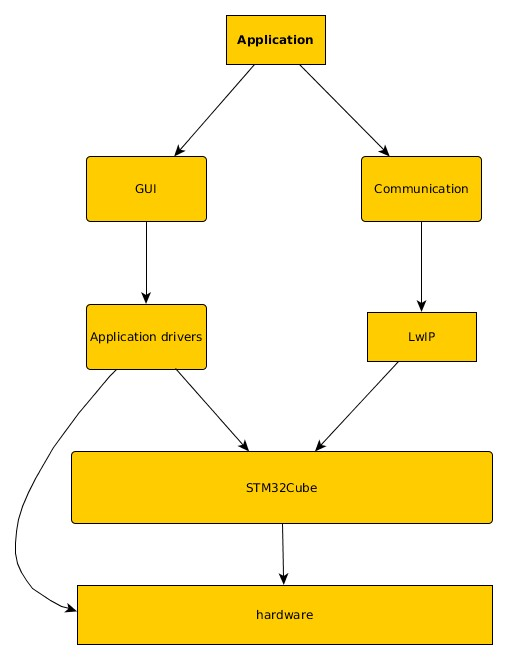
\includegraphics[width=140mm, height=140mm]{../diagrams/stm_fw_struktura.jpg}
\caption{Struktura firmware}
\label{stm-fw-struktura}
\end{figure}

% popis obrázku
Na obrázku (TODO: ref) vidíme strukturu celého firmware rozdělenou do jednotlivých vrstev.
Jednotlivé entity na obrázku odpovídají buď jednomu typu resp. třídě (jako je tomu v případě \texttt{Application}),
nebo skupině tříd, ve které jsou pro ilustraci vypsány některé konkrétní třídy, nebo knihovně.
\texttt{Application} je na nejvyšší úrovni abstrakce a provádí hlavní aplikační logiku.
Jednak přímo pracuje se skupinou tříd \texttt{GUI}, pomocí které zobrazuje uživateli aktuální data
popřípadě mu umožňuje nastavení některých dat, ale také pracuje přímo se skupinou \texttt{Communication},
která obstarává veškerou komunikaci se serverem.
Skupina \texttt{Application Drivers} obsahuje aplikačně specifické wrappery hardware ovladačů nad
\texttt{STM32Cube}, v jednom případě i třídu \texttt{OneWire}, která přistupuje k hardware přímo
a ne přes \texttt{STM32Cube}.
\texttt{STM32Cube} je balíček knihoven tak, jak je zmíněn v kapitole analýza/stm/software.

Obrázek (TODO: ref) slouží pouze jako nástin struktury firmware a nikoli jako detailní popis fungování jednotlivých
typů.
Bližší informace o struktuře skupiny \texttt{Communication} je uvedena v kapitole implementace komunikace (TODO: ref),
struktura skupiny \texttt{GUI} je popsána v kapitole gui (TODO: ref)


\subsection{Tasky}

% Definice tasku
V následujícím textu budeme označovat \emph{task} jako sémanticky samostatné výpočetní
vlákno.
V podstatě je to totéž jako task v kontextu RTOS.
V STM je paralelismus pouze virtuální, protože procesor je jednojádrový.

% Tasky v naší aplikaci
Naše aplikace potřebuje provádět 3 tasky:
\begin{itemize}
  \item \textbf{GUI task} má na starosti periodicky iterovat přes všechny GUI elementy
    na displeji a v případě potřeby je překreslit.

  \item \textbf{User input task} má na starosti zjišťovat jestli uživatel zadal nějaký
    vstup, ať už je to zmáčknutí joysticku, nebo jiného tlačítka.

    Uživatelský vstup lze zpracovávat i pomocí interrupt handlerů - joystick
    ale i jiná tlačítka lze nastavit tak, aby při stlačení vyvolali interrupt.
    Pro naši situaci to ale není výhodné, protože bychom museli mít více různých
    interrupt handlerů pro každý možný vstup.
    Lepší je nastavit periodický task tak, aby iteroval všechny možné vstupy.

  \item \textbf{Ethernet task} má na startosti zpracování paketů z ethernetové
    periferie. Je potřeba periodicky volat dvě funkce z LwIP knihovny -
    \texttt{ethernetif\_input}, která se stará o nízko-úrovňový příjem nebo odesílání paketů resp.
    bajtů z ethernetové periferi, a \texttt{sys\_check\_timeouts}, která kontroluje platnost různých
    dočasných hodnot, jako je třeba ARP tabulka, a v případě potřeby je obnoví.

  \item \textbf{RTC task} má na starosti zpracovávání sekundového interruptu a jednou za
    minutu změřit aktuální teplotu.
\end{itemize}

% Definice mainloop
Vzhledem k tomu, že firmware je jediné, co v STM poběží, je potřeba aby svůj běh neukončil
hned po prvním vykreslení obrazovky resp. zpracování pár paketů.
Potřebovali bychom mít někde ve firmware nekonečný cyklus, který bude zpracovávat naše
tasky.
Takovému nekonečnému cyklu budeme říkat \emph{mainloop}.
V rámci firmware pro embedded zařízení, který nemá RTOS, je použití \emph{mainloop} běžné.

% definice interrupt handler kontextu
Kromě \emph{mainloop} můžou být tasky vykonávané ještě v rámci interrupt handleru některé
periferie, například časovače, nebo stisknutí tlačítka.
Interrupt handlery mají obecně tu výhodu, že jsou spuštěny vždy po určité události -
v případě časovače je to uplynutí periody.

% mainloop vs interrupt kontext
Ne všechny tasky je vhodné provádět v kontextu interrupt handleru.
Například podle dokumentace LwIP není doporučeno volat jakoukoli funkci, která má odesílat
nebo přijímat pakety z interrupt handleru.
Proto je potřeba ethernet task provádět vždy v rámci mainloop.
% User input task je vhodný provádět z interrupt handleru
Naopak user input task je vhodné provádět v rámci interrupt handleru časovače nastaveného
na rozumnou periodu.
Pokud by se totiž měl provádat z mainloop, není jasné jak přesně by měl fungovat, protože čtení
vstupu od uživatele je samo o sobě blokující funkce.

% SW timer
\subsubsection{Softwarové časovače}
Některé komponenty firmwaru musejí být periodicky notifikovány o vypršení určitého časového intervalu.
V podstatě by takové komponenty využili fungování standardního hardwarového časovače.
Vzhledem k tomu, že hardwarových časovačů je omezeně mnoho a jejich inicializace je pro tyto případy zbytečně složitá,
hodí se vytvořit softwarové časovače.
Jejich myšlenka je jednoduchá.
Z \emph{mainloop} kontrolujeme, jestli nedošlo k jejich vypršení a pokud ano, tak zavoláme jejich
\uv{timeout} funkci.
Pomocí funkce \texttt{HAL\_GetTick} můžeme získat aktuální počet tiků systému v milisekundách, takže
implementace softwarového časovače je skutečně jednoduchá.

Příklad použití softwarového časovače je \texttt{MainFrame}, který musí periodicky zjišťovat stav síťového
připojení, aby ho mohl zobrazit uživateli.



\subsection{Eventy}
V této kapitole rozebereme některé důležité události, které mohou v rámci firmware STM vzniknout.

Mezi tyto události patří:
\begin{itemize}
  % IntervalsChangedStmEvent
  \item Změna intervalů na STM.
    Jako reakci na tuto událost by STM mělo nově nastavené intervaly uložit do EEPROM a dále
    tyto intervaly poslat na server v případě, že na serveru jsou nastavené starší intervaly.

  % IntervalsChangedServerEvent
  \item Příjem intervalů ze serveru o které samo STM požádalo. Reakce na tuto událost je
    uložení intervalů do EEPROM.

  % ConnectEvent
  \item Připojení k serveru. Myšleno ne pouze navázané TCP spojení, ale spojení ve smyslu naší
    aplikace tj. server poslal svůj aktuální čas ve formátu timestampu.
    STM reaguje tak, že si právě přijatý timestamp nastaví jako svůj vlastní čas, tedy
    uloží timestamp do RTC.

  % MeasuredTemperatureEvent
  \item Právě naměřená teplota. Tuto hodnotu chceme zobrazit uživateli na STM a také ji poslat
    na server.

  % CommunicationErrorEvent
  \item Chyba síťové komunikace. Toutu chybou máme na mysli v podstatě libovolnou síťovou chybu
    od vypojení ethernetového kabelu až po nemožnost naparsování HTTP response.
    Na tuto událost STM reaguje restartováním celé komunikace.
    Kvůli složitosti implementace nemá vůbec smysl aby si STM pamatovalo, v jakém stavu chyba
    nastala a zkoušelo komunikace restartovat právě od tohoto momentu.

  % Eth-link UP
  \item Zapojení ethernetového kabelu. Jak jsme již zmiňovali v kapitole analýza, uživateli
    dáváme možnost zapojit nebo odpojit ethernetový kabel za běhu aplikace.
    Zapojení ethernetového kabelu by v ideálním případě mělo ihned odstartovat pokus o spojení se serverem
    a výsledek tohoto pokusu oznámit uživateli.
    Připojit se k serveru může STM pouze pokud má uložený klíč v EEPROM.
    Pro přehlednost a jednoduchost aplikace stanovíme ještě další podmínku, která musí být splněna
    před pokusem o připojení k serveru - aktuální obrazovka musí být \texttt{MainFrame}.

  % KeySavedEvent
  \item Nastavení klíče. Tato událost nastává v momentě, kdy je aktuální obrazovka \texttt{KeyFrame},
    a uživatel stiskne tlačítko \uv{submit}.
    STM na to reaguje uložením klíče do EEPROM a také pokusem o připojení k serveru,
    pokud jsou všechny podmínky pro tento pokus splněny.
\end{itemize}

% Všechny eventy jsou předávané do Application
Každá z výše uvedených událostí je reprezentovaná třídou v programu.
Problém s připojením je například reprezentován třídou \texttt{CommunicationErrorEvent}, nastavení
klíče potom třídou \texttt{KeySavedEvent}, apod.
Události mohou být generované v různých částech programu, \texttt{MeasuredTemperatureEvent} je generovaný
například v \texttt{TempController}.
Všechny tyto události musí být po vzniku předány třídě \texttt{Application}, která v tomto případě
slouží jako centrální autorita ošetřující všechny druhy událostí.

% výhody a nevýhody návrhu
Výhoda tohoto návrh je v tom, že reakce na všechny důležité události máme na jednom místě.
Nevýhoda je potom taková, že nesmíme zapomínat události generovat.


\subsection{GUI}

V rámci kapitoly \ref{popis-gui} jsme specifikovali požadavky, které máme na uživatelské
rozhraní.
V této kapitole se detailněji podíváme na implementaci celého GUI.

%\begin{figure}[tbh!]\centering
%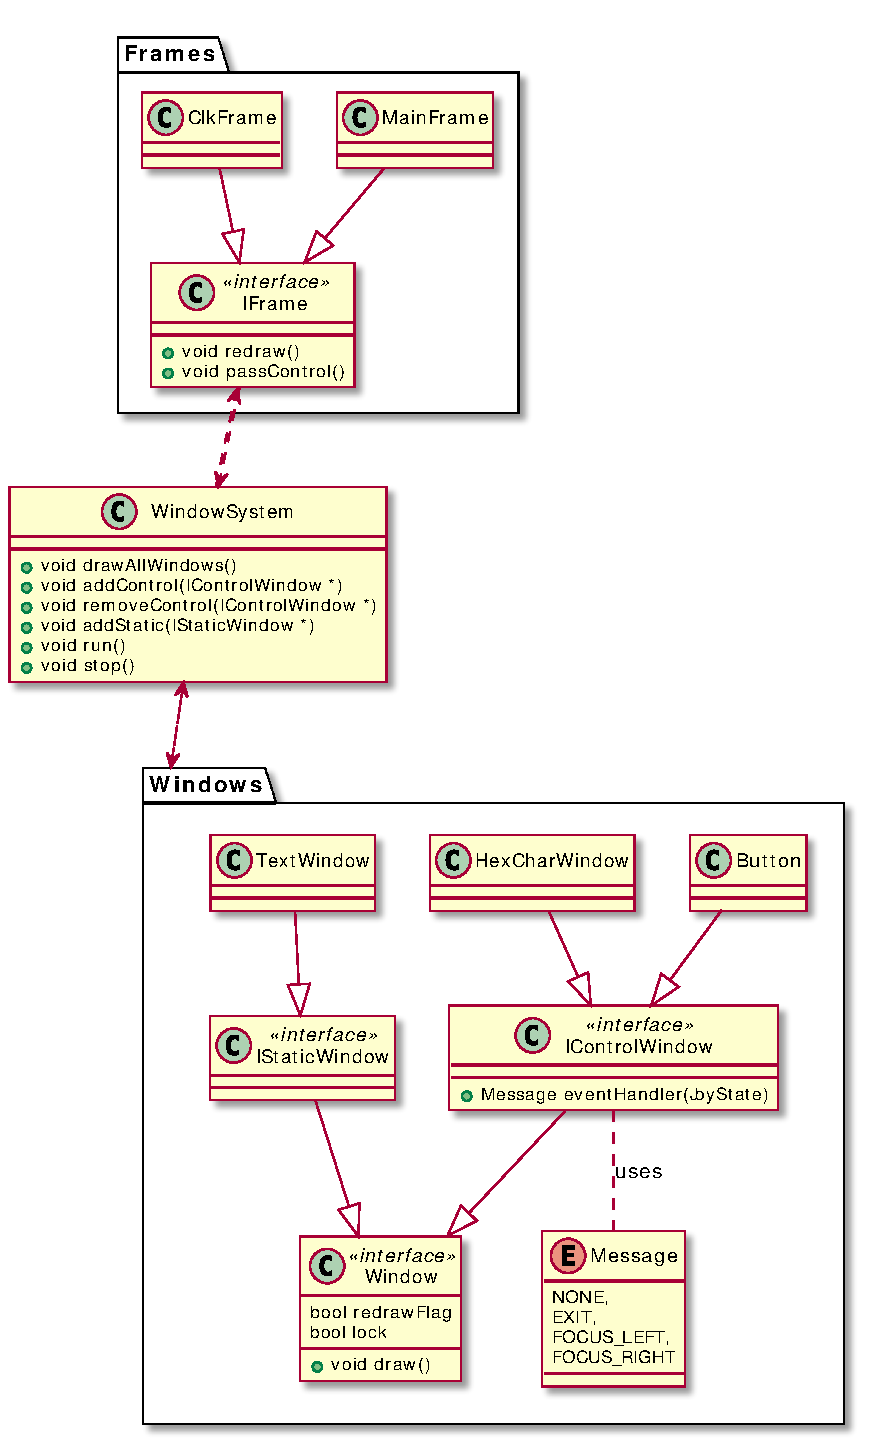
\includegraphics[scale=0.75]{../diagrams/stm_gui.pdf}
%\caption{Hierarchie základních tříd v GUI}
%\label{fig:stm-gui}
%\end{figure}

Obrázek (TODO: odkaz) zobrazuje hierarchii základních tříd a vztahy mezi nimi.
Pro jednoduchost zobrazuje pouze pár konkrétních tříd jako příklad: \texttt{TextWindow} jako statické
okno, které pouze zobrazuje text a \texttt{HexCharWindow} jako kontrolní okno, které je součástí
\texttt{KeyFrame} a zobrazuje právě jeden hexadecimální znak, jehož hodnotu může uživatel
zvětšovat či změnšovat.
Celé GUI je tvořeno dvěma základními druhy objektů - \emph{windows} a \emph{frames}.
Každý frame reprezentuje jednu obrazovku tj. co všechno je v daný moment zobrazeno na displeji.
Windows jsou velice jednoduchá okna - typicky zobrazující pouze neohraničený text resp. číselnou
hodnotu.
Frame obsahuje několik oken a definuje, kde přesně mají tato okna být zobrazena a jakého typu
mají být.
Každý frame má svůj \texttt{WindowSystem}, přes který může sám do sebe vkládat okna.
Kromě toho, že \texttt{WindowSystem} zpracovává vstup, na základě kterého přepíná mezi jednotlivými okny,
funguje také jako prostředník mezi frame a jeho okny.

% Windows
\subsubsection{Windows}
% static and control windows
Window může být buď \emph{statické} (dědí od třídy \texttt{IStaticWindow}), nebo \emph{kontrolní}
(dědí od třídy \texttt{IControlWindow}).
Statické okno slouží pouze pro zobrazování libovolného textu, kontrolní okno může uživatel \uv{nakliknout}
a změnit jeho hodnotu.
Jediný uživatelský vstup je joystick a řekněme, že jeho zmáčknutím doprava nebo doleva se uživatel
přesune mezi jednotlivými okny, a zmáčknutím nahoru nebo dolů může uživatel měnit hodnotu
v právě nakliknutém okně.
Přímé stisknutí joysticku má vliv pouze na okna typu \texttt{Button}, která typicky slouží buď jako
potvrzení všech zadaných hodnot v rámci jedné obrazovky, nebo jako \uv{exit} tlačítko.
Možnost nakliknutí a změny nějaké hodnoty kontrolního okna se do objektového návrhu promítá tak,
že \texttt{IControlWindow} má čistě virtuální metodu \texttt{Message eventHandler(JoyState joyState)}.
Zjednodušeně řečeno každé okno pomocí přetížení této metody specifikuje svoji reakci na vstup,
kde tato reakce může být buď čistě interního charakteru tj. změna hodnot daného okna, nebo může
vrátit jednu z hodnot \texttt{Message::FOCUS\_LEFT} nebo \texttt{Message::FOCUS\_RIGHT}, čímž
říká, že nakliknuté má být kontrolní okno, které je vlevo nebo vpravo od tohoto okna, případně
může vrátit \texttt{Message::EXIT}, čímž říká že má být aktuální frame vypnut.

% WindowSystem
\subsubsection{WindowSystem}
\texttt{WindowSystem} je v podstatě kontejner pro všechna okna v rámci jednoho frame a ještě se stará
o výše zmíněnou logiku.
Frame Při inicializaci pouze přidává kontrolní a statická okna do \texttt{WindowSystem}.
Za běhu potom \texttt{WindowSystem} podle vstupu buď přepíná mezi kontrolními okny, nebo přímo vypne
aktuální frame.

% zpracování vstupu je v interrupt handleru kdežto vykreslování v mainloop
Zde je důležité si uvědomit, že zpracování vstupu probíhá v \emph{user input task}, což je interrupt
handler jednoho z timeru, který tento interrupt spouští jednou za 100 ms.
Z pohledu kódu je tedy zpracování vstupu a všechno s tím spojené asynchronní.
Protože zpracování vstupu běží v jiném kontextu než vykreslování, je potřeba rozlišovat metody podle
toho ve kterém kontextu jsou volány.
Označme metody volané v kontextu zpracování vstupu jako \emph{callback} metody a definujme pro
ně strukturu, kterou rozebereme v následujícím odstavci.

%%%%% Callback metody %%%%%%
\paragraph{Callback metody}
Občas v rámci jednoho frame chceme reagovat na stisknutí některého z čudlíků.
Například při stisku \uv{Exit} v \texttt{SetIntervalFrame} bychom chtěli ukončit celý frame a uložit
uživatelem zadané hodnoty.
Zavedeme několik rozhraní se dvěmi čistě virtuálními metodami: \texttt{callback} a \texttt{register}.
\footnote{Přesný název konkrétních metod se liší, ale callback nebo register je jejich součástí}
\texttt{register} metoda by měla objekt, který chce dostávat callbacky zaregistrovat k jejich zdroji.
\texttt{callback} metoda potom implementuje reakci na konkrétní callback.
Všechny tyto rozhraní dědí od \texttt{ICallbackReceiver}.

Myšlenka je taková, že když chceme, aby objekt A dostával určité callbacky od objektu B,
musíme nejprve objekt A u objektu B registrovat jako \uv{callback receiver} a potom definovat
metodu která na tento callback bude reagovat.

Místo toho, abychom vyjmenovali všechny možné typy callbacků a jejich parametry, zpřesníme
strukturu callback metod na příkladě.

%\begin{figure}[tbh!]\centering
%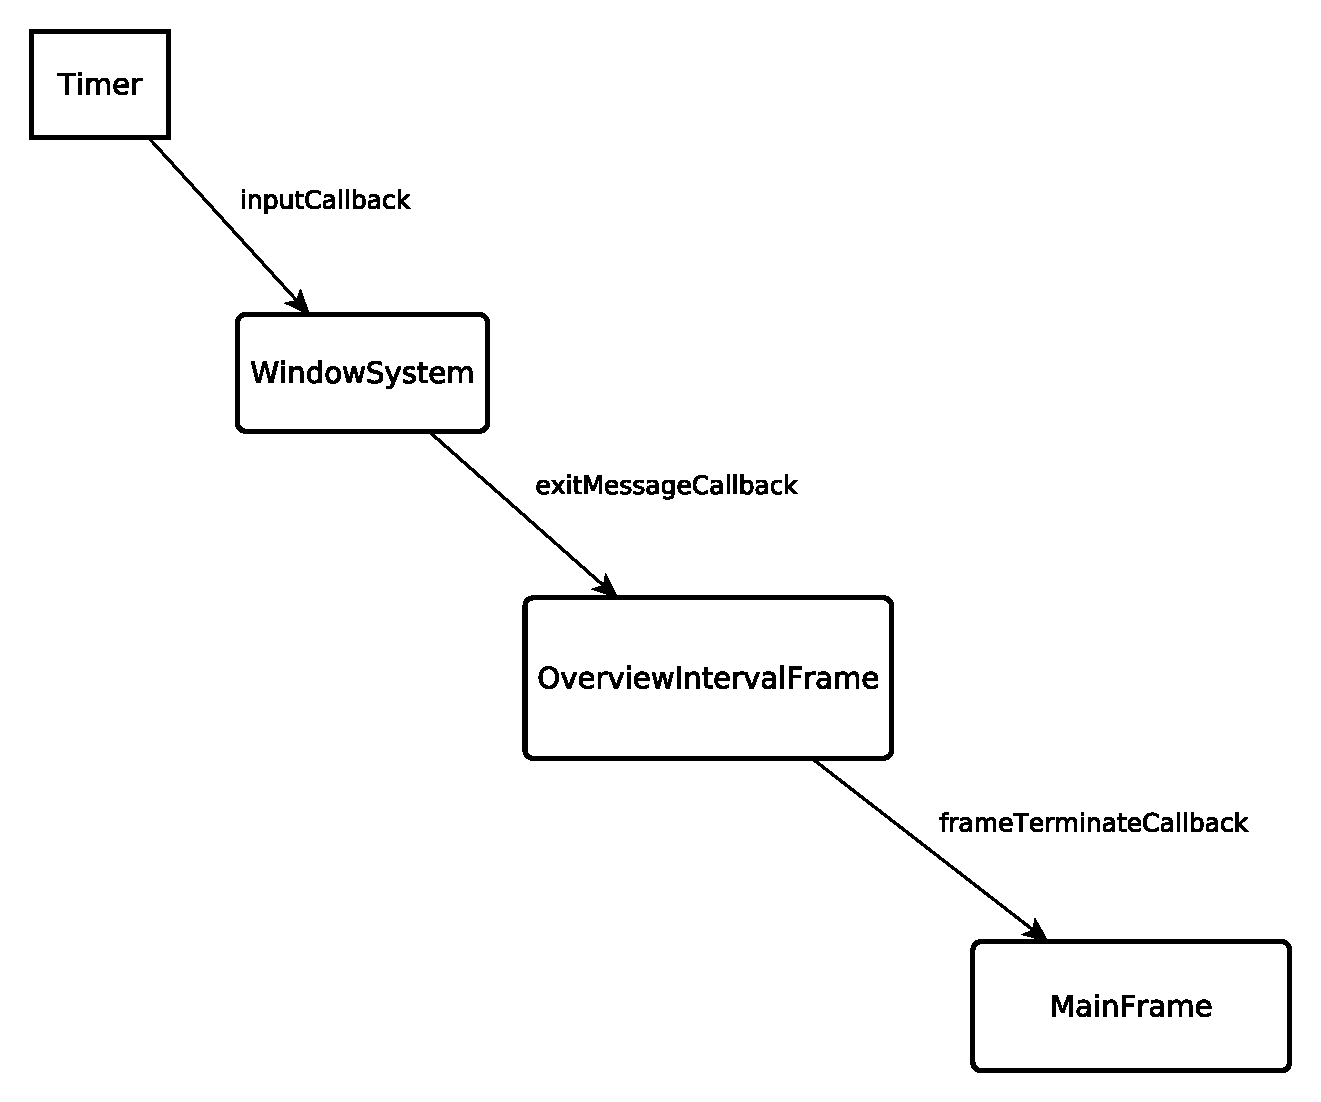
\includegraphics[scale=0.6]{../diagrams/stm_callback_metody.pdf}
%\caption{Příklad hierarchie volání callback metod}
%\label{fig:stm-callback-metody}
%\end{figure}

Diagram (TODO: odkaz) ilustruje situaci, kdy je uživatel v \texttt{OverviewIntervalFrame}, stiskne
tlačítko \uv{exit} a dostane se zpět do \texttt{MainFrame}.
Proces na diagramu je následující:
\begin{enumerate}
  \item Vygenerování interruptu timerem.
  \item Zavolání metody \texttt{IO::task}, ve které dojde k vytvoření callback objektu s parametrem.
  \item Zavolání metody \texttt{WindowSystem::inputCallback}, která tento callback předá aktuálně
    nakliknutému oknu (v tomto případě je to \texttt{exitButton}), které vrátí \texttt{Message::EXIT}
    ze svého \texttt{eventHandler}.
  \item Zavolání metody \texttt{OverviewIntervalFrame::exitMessageCallback}
  \item Zavolání metody \texttt{MainFrame::frameTerminateCallback}, ve které MainFrame určí který
    frame skončil a nastaví sám sebe jako aktuální frame.
\end{enumerate}
%%%%%% konec callback metod %%%%%%%

% přístup k oknům z interrupt handleru/mainloopu --> nutnost zamykání
Celý tento \uv{framework} je navržen s ohledem na co nejsnazší specifikaci vzhledu i chování nově přidávaného
framu, ale také s ohledem na to, že čtení vstupu probíhá v kontextu interrupt handleru, kdežto vykreslování
oken probíhá v \emph{mainloop}.
Mohlo by se tedy stát, že vykreslování okna bude přerušeno, v interrupt handleru se změní jeho hodnoty,
a vykreslování se opět obnoví - toto může vést k tomu, že okno vykreslí špatné hodnoty.
Každé okno má tedy zámek, který je zamčen před voláním metody \texttt{draw} nebo metody \texttt{eventHandler}.
O toto zamykání se nemusí starat programátor při definování nového okna, děje se totiž už na úrovni
třídy \texttt{Window}.

% okna se nepřekreslují, když to není nutné.
Pokud oknu změníme hodnotu a chceme, aby bylo v rámci \emph{GUI task} překresleno, musíme mu explicitně
nastavit \texttt{redrawFlag}.
Díky redrawFlag máme zajištěno i to, že nemusíme zbytečně překreslovat okna, která to nepotřebují.
Přeci jen je vykreslování na displej časově poměrně náročné.



\subsection{Implementace komunikace se serverem}
V této kapitole se detailněji podíváme na implementaci komunikace se serverem.

\begin{figure}[tbh!]
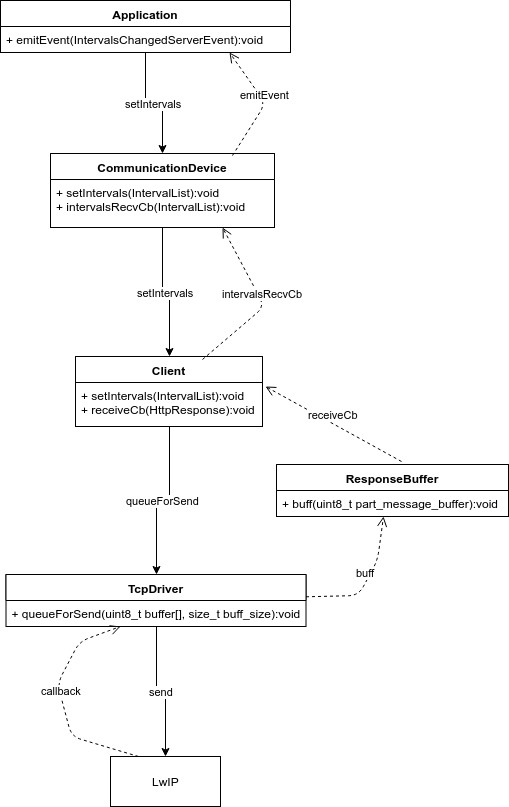
\includegraphics[width=\textwidth, height=600px]{../diagrams/stm_implementace_komunikace.jpg}
\caption{Diagram tříd v rámci komunikace}
\label{stm-implementace-komunikace}
\end{figure}

% popis skupiny Communication
V diagramu \ref{stm-implementace-komunikace} jsou zobrazeny nejdůležitější třídy, vztahy
mezi nimi a zároveň je tam zobrazen i typický proces nastavení intervalů na STM a stažení
intervalů ze serveru, který bude popsán později.
Nejprve popíšeme třídy v diagramu a jejich funkcionalitu.
\begin{itemize}
  \item \texttt{CommunicationDevice} který je objektovou reprezentací samotného STM a \texttt{Application}
    do něj ukládá naměřenou teplotu pro odeslání na server a intervaly pro výměnu se serverem.
    CommunicationDevice notifikuje Application o dvou důležitých událostech - ConnectedEvent a
    IntervalsChangedServerEvent - tedy připojení k serveru a přijetí intervalů ze serveru.
  \item \texttt{Client} je HTTP klientem specifickým pro naše použití. Jednak do něj CommunicationDevice
    přeposílá data, které má od Application, a jednak Client notifikuje CommunicationDevice o
    důležitých událostech týkajících se komunikace se serverem jako jsou: \uv{intervaly byly odeslány},
    \uv{teplota byla odeslána}, \uv{intervaly byly přijaty}, apod.
  \item \texttt{TcpDriver} je wrapper pro LwIP knihovnu.
  \item \texttt{ResponseBuffer} reprezentuje buffer pro HTTP odpovědi ze serveru. \\
    TcpDriver přeposílá vše, co přijme, do ResponseBuffer.
    Ten si tato data ukládá dokud nedostane celou HTTP zprávu.
    Typicky se totiž stává, že server neodešle celou HTTP odpověď v jednom paketu a proto je potřeba
    jednotlivé pakety ukládat a později z nich poskládat celou HTTP odpověď.
    V momentě, kdy ResponseBuffer má celou odpověď, notifikuje o tom Clienta.
    ResponseBuffer také potřebuje vědět jestli očekávaná odpověď od serveru má mít i tělo nebo pouze
    HTTP hlavičku.
\end{itemize}

% popis vztahů
Směrem dolů od Application až po LwIP probíhá odesílání dat na server resp. zařazení těchto dat
do interních front LwIP - k samotnému odeslání dat typicky dojde později.
Směrem nahoru od LwIP, přes TcpDriver, ResponseBuffer až po Application probíhá příjem dat ze serveru.
Z pohledu kódu se dá směr dolů považovat za \uv{synchronní} a směr nahoru za \uv{asynchronní}, proto
jsou také všechny metody, které jsou volané směrem nahoru, definovány jako callback metody.

% popis procesů znázorněných na diagramu
Na diagramu jsou znázorněny dva typické procesy:

\paragraph{Posílání intervalů na server}
Proces probíhající směrem dolů bychom mohli nazvat jako \uv{uložení intervalů do interních
struktur Clienta k budoucímu porovnání s intervaly serveru} (porovnávat se ve skutečnosti bude
pouze timestamp intervalů).
Jakmile se intervaly dostanou do Clienta, musí zde Client počkat, dokud se jeho \emph{komunikační cyklus}
(zmíněný dále v této kapitole) nedostane do stavu, ve kterém porovnává timestamp svých intervalů
a timestamp intervalů ze serveru.
Nezávisle na tom, jak toto porovnání dopadne, musí Client poslat buď GET request, nebo POST request
na server přes TcpDriver.

\paragraph{Příjem intervalů ze serveru}
Je proces probíhající směrem nahoru.
LwIP předává přijatý payload TCP paketů do TcpDriver, který ho dále předává do ResponseBuffer.
Jak již bylo zmíněno, ResponseBuffer postupně ukládá části HTTP odpovědi, dokud nesestaví celou,
potom notifikuje Client pomocí callback metody.
ResponseBuffer už HTTP odpověď naparsoval a Client na základě toho, v jakém stavu \emph{komunikačního cyklu}
se nachází, notifikuje CommunicationDevice (na diagramu notifikuje CommunicationDevice o přijetí
intervalů ze serveru pomocí callback metody \texttt{intervalsReceivedCb}).
CommunicationDevice dále vygeneruje \texttt{IntervalsChangedServerEvent} a pošle do Application
k následnému šíření.

% Client
\subsubsection{Client}
Kromě toho že Client je HTTP klientem, musí také být implementován tak, aby byl kompatibilní s LwIP
callback API.

\begin{figure}[tbh!]\centering
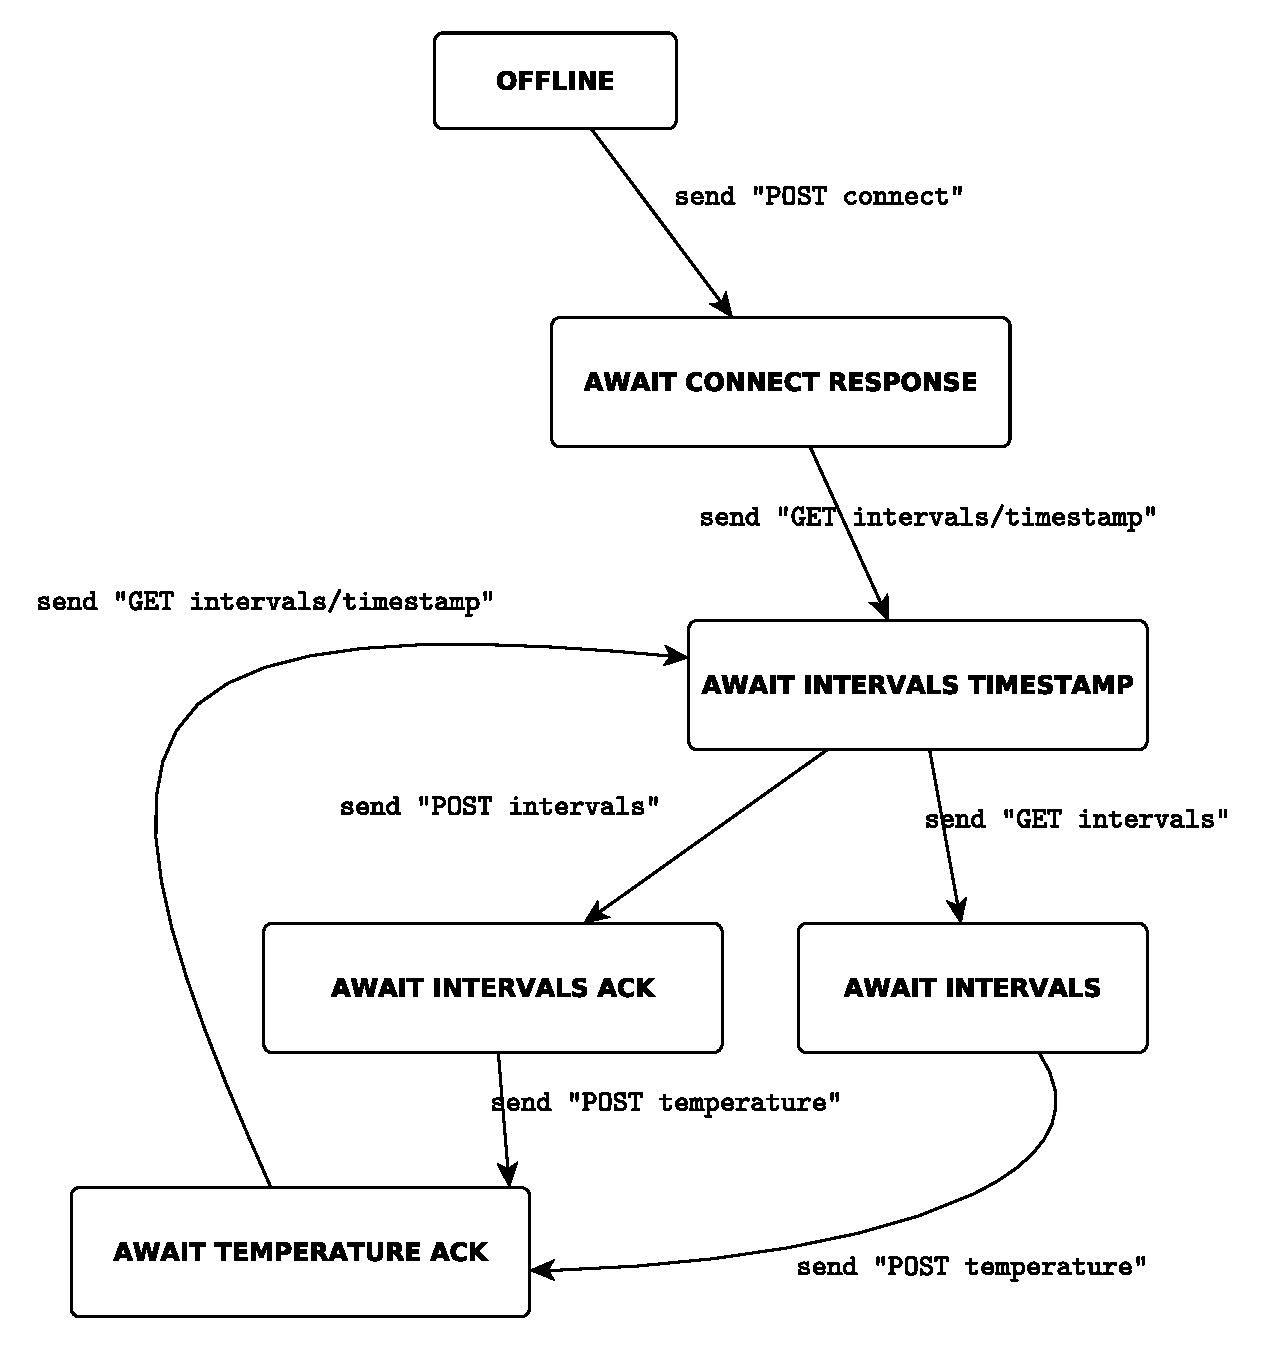
\includegraphics[width=\textwidth, height=150mm]{../diagrams/stm_komunikacni_cyklus.pdf}
\caption{Komunikační cyklus}
\label{stm-komunikacni-cyklus}
\end{figure}

Na diagramu \ref{stm-komunikacni-cyklus} je znázorněn \emph{komunikační cyklus} a jednotlivé stavy tohoto cyklu.
Zjednodušeně řečeno se v rámci celého cyklu nejprve buď pošlou intervaly na server nebo stáhnou ze
serveru - záleží na tom, jestli má STM větší timestamp než server - poté se pošle teplota na server.
Pokud cyklus probíhá poprvé, musí se nejprve STM k serveru přihlásit.
Celý cyklus je opakován v určitých časových intervalech.
\footnote{Konkrétně jsou to 2 sekundy, je pro to použit softwarový časovač}

% Ošetření chyb
Mezi libovolnými dvěma stavy může dojít k chybě.
Chyby ošetříme tak, že celý cyklus restartujeme od stavu \texttt{OFFLINE}.
Mohli bychom sice uložit stav před chybou a po zpracování chyby pokračovat opět od tohoto stavu,
bylo by to ale příliš komplikované.
Navíc v našem případě je během celého cyklu přeneseno relativně malé množství dat, takže restartování
od úplného začátku nás skoro nic nestojí.




\subsection{EEPROM}
EEPROM používáme jako persistentní datové uložiště, do kterého ukládáme konfiguraci intervalů
a privátní DES klíč.
Kromě samotných intervalů a samotného klíče je ještě potřeba do EEPROM ukládat metadata -
například počet intervalů, timestamp intervalů nebo flag značící jestli klíč je uložen.
Je zbytečně složité kvůli těmto pár datům a metadatům používat nějaký file systém.

% Detaily implementace
Co se týká implementačních detailů, tak \texttt{EEPROM} je třída, která se stará o ukládání
dat do EEPROM a mimo jiné obsahuje definice adres, na které jsou ukládány různá data a metadata.
EEPROM při inicializaci nevyžaduje žádný specifický formát, což mimo jiné znamená, že vymazat
všechna data z EEPROM znamená vyplnit celou EEPROM nulami.

Vymazání celé EEPROM je také něco, co je vhodné udělat předtím než se uživatel STM rozhodne
toto zařízení předat někomu jinému.




\section{Webový server}

% TODO: obrázek

Webový server je rozdělený do dvou na sobě nezávislých komponent \texttt{user\_interface} a
\texttt{stm\_communication} tak, jak je to znázorněno na obrázku (TODO: ref).
\texttt{user\_interface} zprostředkovává veškerou komunikaci mezi uživatelem (klientem) a jeho STM
zařízeními sestávající z nastavování intevalů a čtení aktuálně naměřené teploty.
\texttt{stm\_communication} přijímá aktuálně naměřenou teplotu od STM zařízení a vyměňuje si s nimi intervaly.
Obě komponenty čtou a zapisují data do společné databáze.
Tím je nepřímo zajištěna komunikace mezi uživatelem a jeho zařízením skrz server.

% Použití frontend frameworku by bylo vhodné.
V kapitole analýza jsme se rozhodli použít Django jako backend framework, k vývoji frontend
používáme pouze Bootstrap a jQuery.
Vzhledem k požadované interaktivitě frontend jsme si tímto rozhodnutím trochu zkomplikovali práci.
Kdybychom chtěli přidat další funkcionalitu, jako je například zobrazení historie pro STM,
bylo by vhodné do serveru integrovat nějaký frontend framework.

Samotná implementace frontend není pro tuto práci příliš důležitá, proto se jí zabývat nebudeme.
Implementace backend už důležitá je, ovšem v porovnání s implementací STM, kde na serveru máme
k dispozici velikou abstrakci, máme zjednodušenou práci.

% Databázové schéma
\subsection{Databázové schéma}

\begin{figure}[tbh]\centering
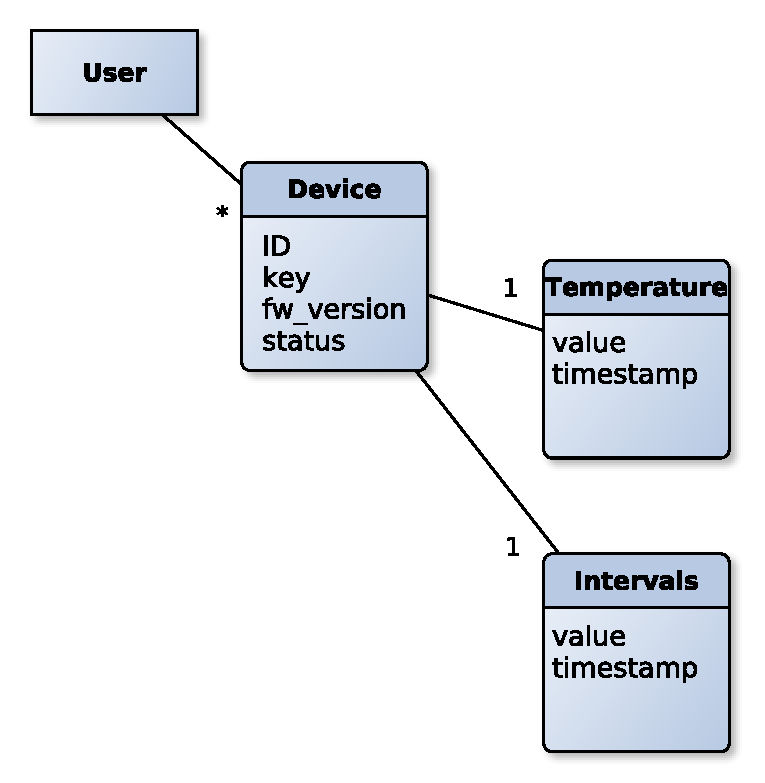
\includegraphics[scale=0.8]{../diagrams/databazove_schema.pdf}
\caption{Databázové schéma}
\label{databazove-schema}
\end{figure}

Databázové schéma \ref{databazove-schema} ukazuje základní objekty a vztahy mezi nimi.

Na server se může registrovat libovolný uživatel zadáním uživatelského jména, hesla a potvrzením
emailové adresy.
Každý uživatel si může přidat omezeně mnoho zařízení.
%TODO: footnote: Proces přidání nového zařízení a s tím související vygenerování klíče serverem a zadání tohoto klíče
%  do STM je popsán v kapitole (TODO: ref práce-se-systémem).
Každé STM zařízení má svoje ID přiřazeno ještě před tím, než se dostane uživateli do ruky.
Kromě toho, že toto ID je uloženo v databázi na serveru, je potřeba aby bylo zakódovano do firmware
konkrétního STM, což by neměl být problém.
Každé STM má také přiřazenou verzi firmware, to z důvodu že by STM mohlo být teoreticky aktualizováno
na dálku (TODO: odkaz), server, ani STM toto ale zatím nepodporují.
\texttt{status} může být buď \texttt{connected} nebo \texttt{offline}.
\texttt{key} se k STM přiřadí až po tom, co se poprvé přihlásí k serveru.

Co se týká jednotlivých položek, v našem případě \texttt{Temperature} a \texttt{Intervals}, tak ty se
dělí na dva typy - \emph{actual} a \emph{config}.
Actual položky jsou takové, které STM periodicky posílá na server a ten má za úkol je zobrazit uživateli.
Config položky nejsou pouze ke čtení a i k zápisu.
Tak, jak je to zmíněno v kapitole (TODO: ref analýza/komunikace), jsou config položky synchronizovány mezi
serverem a STM tak, že na obou stranách platí pouze hodnota s novějším timestampem.
Každá položka v databázi má svůj timestamp a \texttt{value}.
Temperature představuje teplotu, tedy jeho value je prostě číslo.
Na druhou stranu Intervals představuje nastavení teplot po různé časové intervaly, což znamená, že ve
value musí být uložená nějaká komplikovanější hodnota než je číslo.
Vhodné řešení je ukládat do intervals textový řetězec v JSON formátu, zejména kvůli tomu, že v rámci
Pythonu a Javascript se JSON řetězec velice jednoduše parsuje.




\section{Komunice STM a web serveru}
\subsection{Specifikace HTTP zpráv}

Tato sekce probírá detaily HTTP komunikace mezi STM a webovým serverem.

% Connection fáze
\subsubsection{Fáze připojování}
Nejprve je potřeba vyřešit připojení STM k serveru.
Chceme totiž uživateli dát vědět zda je STM k serveru připojené a uživatel může tím pádem
sledovat aktuálně naměřené hodnoty přes web.

Můžeme poslat požadavek typu:
\begin{packetstm}
POST /controllers/connect
Content-Type: text/plain

<device_id>
\end{packetstm}

\begin{packetserver}
HTTP/1.1 200 OK
[options]

<server_real_time>
\end{packetserver}

\texttt{server\_real\_time} je timestamp odeslaný serverem sloužící k synchronizaci času
mezi STM a serverem (odkaz).

% Posílání naměřené teploty
\subsubsection{Odesílání naměřené teploty}
\begin{packetstm}
POST /actual/temp
Content-Type: text/plain

<temp_timestamp>
<temp_float>
\end{packetstm}

Kde \texttt{temp\_timestamp} je \texttt{timestamp} značící kdy byla teplota naměřena a
\texttt{temp\_float} je teplota v desetinné přesnosti.

% Výměna intervalů
\subsubsection{Výměna intervalů}
\begin{packetstm}
GET /config/intervals/timestamp
\end{packetstm}

\begin{packetserver}
HTTP/1.1 200 OK
[options]

<interval_timestamp>
\end{packetserver}

STM porovná přijatý \texttt{interval\_timestamp} se svým \texttt{timestampem} a pokud má novější nastavení než server,
tak je odešle:
% odesílání intervalů
\begin{packetstm}
POST /config/intervals
Content-Type: application/octet-stream

<intervals_timestamp>
<intervals>
\end{packetstm}

pokud má starší nastavení než server, tak si je od serveru vyžádá:
% přijímání intervalů
\begin{packetstm}
GET /config/intervals
\end{packetstm}

\begin{packetserver}
HTTP/1.1 200 OK
Content-Type: application/octet-stream
[options]

<intervals>
\end{packetserver}

\paragraph{Formát intervalů}
je následující (stejný jako formát, ve kterém si samo STM intervaly ukládá do své EEPROM)
\texttt{<from>} \texttt{<to>} \texttt{<temp>}, kde \texttt{from} a \texttt{to} jsou
časy v sekundách v rámci dne a \texttt{temp} je teplota.
Každá položka reprezentuje 4 bajtové neznaménkové číslo.



\chapter*{Závěr}
\addcontentsline{toc}{chapter}{Závěr}

Cíle práce se dají rozdělit do tří částí: embedded část práce, web-server část práce a nakonec
komunikace mezi webový serverem a embedded zařízením.
Dále shrneme jakým způsobem jsme dosáhli cíle v rámci jednotlivých částí.

\paragraph{Embedded část práce}
V rámci této části práce jsme měli za cíl vytvořit firmware umožňující uživateli nastavovat
různé teploty po různé časové úseky během dne a zároveň zobrazovat aktuálně naměřenou teplotu.
Jako embedded zařízení jsme zvolili STM3210C-Eval board a firmware vytvořili pomocí knihoven
od STM tak, aby byl přenositelný na de-facto libovolné STM32 zařízení.
Vzhledem k náročnosti programování v embedded prostředí jsme zvolili strategii udržet firmware
co nejjednodušší.
Specifikovali jsme několik různých obrazovek, které může STM3210C-Eval board zobrazovat na svém
displeji a díky kterým může uživatel nastavit jednotlivé intervaly, vidět aktuálně naměřenou teplotu a
připojit zařízení k serveru.

\paragraph{Část práce zabývající se webovým serverem}
Vzhledem k povaze embedded zařízení a požadavku na co nejjednodušší firmware, jsme se rozhodli
implementovat webový server jako separátní entitu.
Přestože námi implementovaný webový server nemá příliš rozsáhlou funkcionalitu, mohl by do budoucna
být rozšířen o spoustu dalších vlastností.

\paragraph{Komunikace mezi serverem a embedded zařízením}
V rámci této části práce jsme rozebrali několik možností, jak by šla komunikace mezi webový serverem
a embedded zařízením realizovat.
Nakonec jsme se rozhodli pro implementaci komunikace pouze pomocí HTTP.
Specifikace komunikace by mohla být snadno rozšířena o několik dalších položek, aniž by se měnil její
princip.
Dále jsme rozebrali možnosti jak komunikaci zabezpečit a to jak ve smyslu autentizace STM na serveru,
tak ve smyslu "skrytí" obsahu komunikace pomocí šifrování.


% shrnutí
\paragraph{Shrnutí}
Přestože v rámci této práce podporujeme "pouze" STM32 zařízení, které serveru posílá pouze naměřenou
teplotu a vyměňuje si s ním nastavení časových intervalů, do specifikace komunikace by se poměrně
snadno daly zařadit i další položky jako je například vlhkost vzduchu.
Dodejme, že pro podporu jiných embedded zařízení by bylo potřeba přeprogramovat hardware-specifickou
část firmware, nicméně na serveru by přidání podpory pro nový typ zařízení nebylo složité.

% použití RTOS a GUI knihovny

%%% Seznam použité literatury
%%% Seznam použité literatury (bibliografie)
%%%
%%% Pro vytváření bibliografie používáme bibTeX. Ten zpracovává
%%% citace v textu (např. makro \cite{...}) a vyhledává k nim literaturu
%%% v souboru literatura.bib.
%%%
%%% Příkaz \bibliographystyle určuje, jakým stylem budou citovány odkazy
%%% v textu. V závorce je název zvoleného souboru .bst. Styly plainnat
%%% a unsrt jsou standardní součástí latexových distribucí. Styl czplainnat
%%% je dodáván s touto šablonou a bibTeX ho hledá v aktuálním adresáři.

% \bibliographystyle{czplainnat}    %% Autor (rok) s českými spojkami
% \bibliographystyle{plainnat}    %% Autor (rok) s anglickými spojkami
 \bibliographystyle{unsrt}       %% [číslo]

\renewcommand{\bibname}{Seznam použité literatury}

%%% Vytvoření seznamu literatury. Pozor, pokud jste necitovali ani jednu
%%% položku, seznam se automaticky vynechá.

\bibliography{literatura}

%%% Kdybyste chtěli bibliografii vytvářet ručně (bez bibTeXu), lze to udělat
%%% následovně. V takovém případě se řiďte normou ISO 690 a zvyklostmi v oboru.

% \begin{thebibliography}{99}
%
% \bibitem{lamport94}
%   {\sc Lamport,} Leslie.
%   \emph{\LaTeX: A Document Preparation System}.
%   2. vydání.
%   Massachusetts: Addison Wesley, 1994.
%   ISBN 0-201-52983-1.
%
% \end{thebibliography}


%%% Obrázky v bakalářské práci
%%% (pokud jich je malé množství, obvykle není třeba seznam uvádět)
\listoffigures

%%% Tabulky v bakalářské práci (opět nemusí být nutné uvádět)
%%% U matematických prací může být lepší přemístit seznam tabulek na začátek práce.
\listoftables

%%% Použité zkratky v bakalářské práci (opět nemusí být nutné uvádět)
%%% U matematických prací může být lepší přemístit seznam zkratek na začátek práce.
\chapwithtoc{Seznam použitých zkratek}

%%% Přílohy k bakalářské práci, existují-li. Každá příloha musí být alespoň jednou
%%% odkazována z vlastního textu práce. Přílohy se číslují.
%%%
%%% Do tištěné verze se spíše hodí přílohy, které lze číst a prohlížet (dodatečné
%%% tabulky a grafy, různé textové doplňky, ukázky výstupů z počítačových programů,
%%% apod.). Do elektronické verze se hodí přílohy, které budou spíše používány
%%% v elektronické podobě než čteny (zdrojové kódy programů, datové soubory,
%%% interaktivní grafy apod.). Elektronické přílohy se nahrávají do SISu a lze
%%% je také do práce vložit na CD/DVD. Povolené formáty souborů specifikuje
%%% opatření rektora č. 72/2017.
\appendix
\chapter{Přílohy}

\section{První příloha}

\openright
\end{document}
